\subsubsection{\stid{1.09} Distributed Tasking at Exascale: PaRSEC}


\paragraph{Overview}

The PaRSEC Environment provides a software ecosystem composed of a runtime
component to dynamically execute task-based applications on heterogeneous
distributed systems, and a productivity toolbox that comprises a development
framework for the support of multiple Domain Specific Languages (DSLs) and
extensions, with debugging, trace collection, and analysis tools.
%
\begin{wrapfigure}[17]{l}{.45\linewidth}
\includegraphics[scale=0.3]{projects/2.3.1-PMR/2.3.1.09-ParSEC/PaRSEC-diagram.png}
\caption{PaRSEC\label{fig:parsec} modular framework allows each
component to be dynamically activated.}
\end{wrapfigure}
%
The PaRSEC project team is dedicated to solving two challenging and
interdependent problems facing the ECP developer community: First, how to create
an execution model that enables developers to express as much parallelism as
possible in their applications, so that applications effectively utilize the
massive collection of heterogeneous devices ECP machines will deploy. Second,
how to ensure the execution model is flexible and portable enough to actually
provide and sustain a performance benefit by increasing the scientific
productivity of the application developers, not only for the ECP target
environments but for the foreseeable future.

PaRSEC is an open source, community-based implementation of a generic task-based
runtime that is freely available, and used by an increasing number of software
libraries.
%  The PARSEC development team is mainly comprised of research staff at % UTK,
%  but regular contributions from the community are provided via our presence %
%  on GitHub and Bitbucket.
The project focuses on providing a stable and efficient infrastructure for quick
prototyping of different approaches to define task-based languages able to
exploit the full range of capabilities of Exascale platforms. Without such a
project, and based on the current state of task-based runtimes, potential users
will be stuck either in fixed programming paradigms, or with a particular,
potentially less efficient, mix of programming languages. The DTE project
provides means to maintain a high competitiveness in the field leading to more
innovation on addressing the challenges we are facing toward scalable,
efficient and Exascale-ready programming paradigms.

\paragraph{Key Challenges}
%\textit{Describe what is hard to do, why it is challenging.}

As Exascale platforms delivery become a closer deadline, an increasing number of
aspects of the hardware and software environment still pose challenges. First
and foremost, keeping pace with the architectural changes on current and future
platforms requires changes not only on how we take advantage of the hardware
capabilities, but how we reshape our algorithms and applications to expose
enough parallelism to maximize the use of the underlying hardware. The number of
nodes, threads per node, memory hierarchies and support for increased
computational capabilities (accelerators) will continue to increase, while the
currently available programming paradigms are still struggling with parallelism
at the node level.

\begin{wrapfigure}{l}{.45\linewidth}
\centering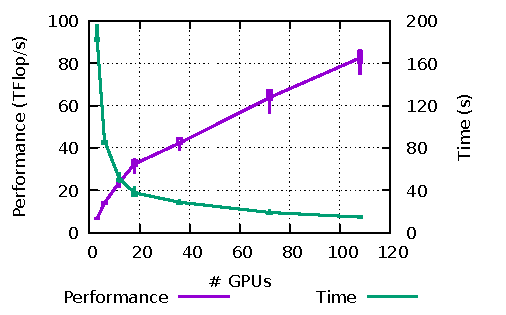
\includegraphics[width=.9\linewidth]{projects/2.3.1-PMR/2.3.1.09-ParSEC/irr-bs-gemm-combined.pdf}
\caption{Time to solution and Performance as a function of the number
  of V100 GPUs on Summit, for the molecule
  $C_{65}H_{132}$\label{fig:irrbsgemm}}
\end{wrapfigure}\paragraph{Solution Strategy}
%\textit{Describe your basic strategy for addressing the challenges.}
The approach followed in PaRSEC is to provide a low-level, flexible and dynamic
runtime able not only to schedule tasks at the node level, but to handle data
transfers between different memory (both inter- and intra-nodes), memory
hierarchies, heterogeneous architectures with support for accelerators with a
simple programming scheme. The proposed approach envisions a middle-ground
solution, addressing both hardware and software challenges. At the hardware
level a team of dedicated developers extends PaRSEC to map its capabilities to
the hardware and to improve its scalability and performance. At the upper
software level the runtime interactions are through Domain Specific Languages
with the target domain scientists in mind, that will facilitate the expression
of algorithmic parallelism with familiar constructs mapped on the exposed
low-level capabilities. To facilitate the integration of PaRSEC-driven libraries
into larger and complex applications, PaRSEC natively interoperate with other
programming paradigms, including some target of the ECP PMR support, such as
PGAS, MPI, OpenMP and Kokkos. This integration provides a smooth transition for
library developers that embrace the PaRSEC runtime, providing a platform where a
shift to a new programming paradigms can be done in stages of increased
complexity~\cite{lorapo-protools,BLR_LU,parsec_pdgemm}.
% In this model, PaRSEC remains in full control of data tracking and
% allocation on the managed accelerator.


%
% Recent work: irregular block-sparse GEMM on Summit
%


The PaRSEC team, in collaboration with NWChemEx project researchers,
developed an efficient and portable tensor product algorithm
specifically designed for the computational chemistry domain needs on
top of the PaRSEC runtime. This includes an efficient matrix product
operation for hybrid architectures, like Summit, with an irregularly
blocked, block-sparse representation of matrices. Moreover, the
requirements on this implementation were extremely strict, the
matrices are rectangular and extremely large in at least one of their
dimensions, such that none of the input matrices could fit in the
aggregated memory of all GPUs. The algorithm and a deeper analysis of
the results are described in~\cite{parsec::rr::irrbs}.

\begin{wrapfigure}[16]{l}{.45\linewidth}
\vspace*{-2em}\centering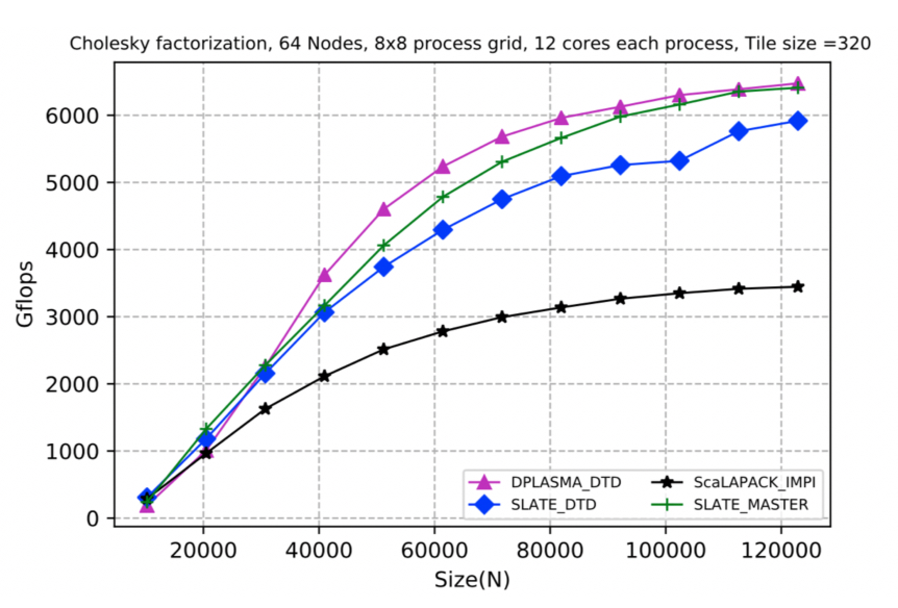
\includegraphics[scale=0.50]{projects/2.3.1-PMR/2.3.1.09-ParSEC/slate_updated_nacl.pdf}
  \caption{Comparison of DPLASMA and SLATE Cholesky factorization over PaRSEC with
           SLATE and ScaLAPACK on 64 nodes 12 cores each\label{fig:slate-parsec}}
\end{wrapfigure}
Figure~\ref{fig:irrbsgemm} shows a strong scaling performance
evaluation of this algorithm, when applied to the main tensor product
required by the CCSD method to simulate the electronic structure from
first principles. The simulated molecule was $C_{65}H_{132}$, which is
a quasi-1-dimensional system and small atomic orbital basis, where the
sparsity of tensors is maximized while the optimal (from the data
compression perspective) tile size is small. That molecule is
representative of applications to 1-d polymers and quasi-linear
molecules (such as some proteins), while the choice of the atomic
orbital basis is representative of medium-precision simulations in
chemistry and condensed phase. Such use case stresses the system and
algorithm as it implies a significant sparsity: the largest matrix,
while being of square of rank $2,464,900$, has only a density of
3.1\%.

The strong scaling evaluation shows a parallel efficiency of 35\%,
with a time to solution at 180s on 3 GPUs, going down to 13s at 118
GPUs.
% The performance per GPU decreases with the number of nodes,
% between 36\% at 3 GPUs and 12\% at 118 GPUs.
Compared to the state of the art, DBCSR~\cite{parsec::dbcsr} can only
run problems that fit in the GPU memory, preventing us to run the same
experiment, but experiments on synthetic problems that fit in memory
show an improvement by a factor two, while
TiledArray~\cite{parsec::tiledarray} cannot leverage the GPUs of
Summit without using PaRSEC and would run, on the CPUs of Summit ten
times slower.
%
% End
%


An important aspect of the DTE project is to define and prototype scalable
domain specific languages that enable a productive expression of parallelism for
end-user communities. PaRSEC presents multiple programming interfaces
(Parameterized Task Graphs for maximum parallelism, the popular serial task
insertion dataflow model to provide direct access to the runtime). In addition,
the DTE team is in close contact with application teams to define parallel
abstractions that are suitable for their domain usage. Notably, the PaRSEC team
has ongoing collaboration with the SLATE linear algebra package and NWChemEx and
GAMESS chemistry package teams.

In this context it is interesting to highlight the first step toward
the integration of the PaRSEC framework into the SLATE (2.3.3.09) in
the context of the shared milestone (STPM11-23). The first prototype
of the application ran in a distributed environment and showed the
capability of the SLATE library using a modern fully capable runtime
system. This work involved enhancing the insert task interface
available in the ParSEC runtime to map onto the logic of a SLATE
algorithm.

Figure~\ref{fig:slate-parsec} compares different implementation of the
Cholesky factorization. On one side we have two reference
implementation for distributed linear algebra, ScaLAPACK and the
current version of the SLATE library (using OpenMP for intra-node
parallelism and MPI for communications). On the other side we have two
DSL expressing the same algorithm but using PaRSEC as the underlying
runtime, the Dynamic Task Discovery (DTD) an approach similar to
OpenMP but working on a distributed setting, and a version of the
SLATE library where instead of relying on explicit parallelism
(OpenMP) and communications (MPI) it rely on implicit dependencies
management via PaRSEC.


% side including the integration of SLATE and PaRSEC. Two domain
% specific languages that have the capability to do linear algebra; then
% against the regular SLATE using OpenMP for intra-node parallelism, and
% MPI for communication; and finally against ScaLAPACK, which is the
% reference for distributed linear algebra.

%
% Recent work: ScaLAPACK - DPLASMA - PaRSEC
%


%\begin{wrapfigure}{l}{.42\linewidth}
%\centering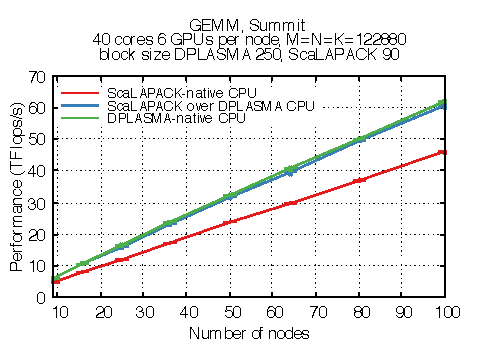
\includegraphics[width=.9\linewidth]{projects/2.3.1-PMR/2.3.1.09-ParSEC/scalapack_cpu_GEMM.pdf}
%\centering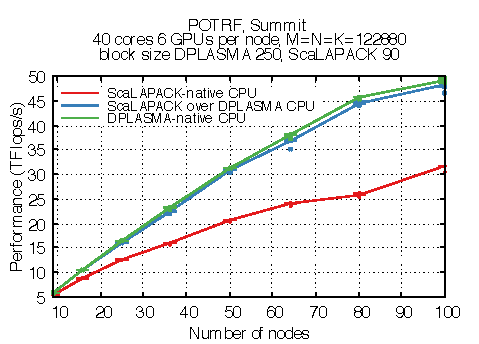
\includegraphics[width=.9\linewidth]{projects/2.3.1-PMR/2.3.1.09-ParSEC/scalapack_cpu_POTRF.pdf}
%\caption{Performance using only CPUs of native ScaLAPACK, ScaLAPACK
%  over DPLASMA and native DPLASMA for GEMM and
%  POTRF.\label{fig:scalapack_cpu}}
%\end{wrapfigure}
%\begin{wrapfigure}{l}{.42\linewidth}
%\centering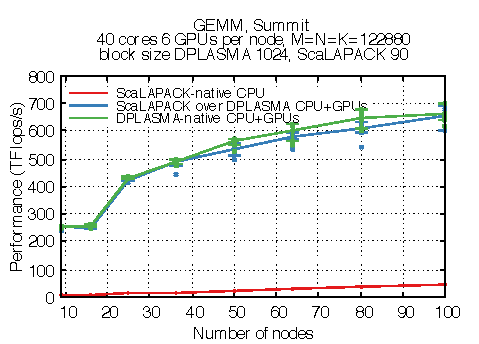
\includegraphics[width=.9\linewidth]{projects/2.3.1-PMR/2.3.1.09-ParSEC/scalapack_gpu_GEMM.pdf}
%\centering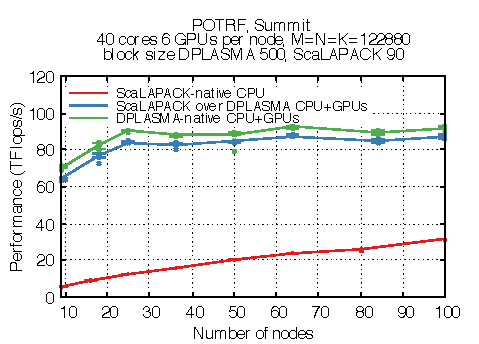
\includegraphics[width=.9\linewidth]{projects/2.3.1-PMR/2.3.1.09-ParSEC/scalapack_gpu_POTRF.pdf}
%\caption{Performance using GPUs of native ScaLAPACK, ScaLAPACK over
%  DPLASMA and native DPLASMA for GEMM and
%  POTRF.\label{fig:scalapack_gpu}}
%\end{wrapfigure}
\begin{wrapfigure}{l}{.45\linewidth}
\centering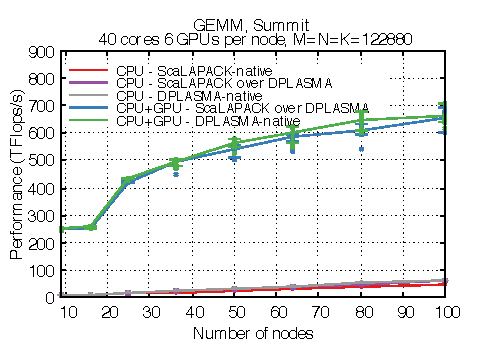
\includegraphics[width=.9\linewidth]{projects/2.3.1-PMR/2.3.1.09-ParSEC/scalapack_GEMM.pdf}
\centering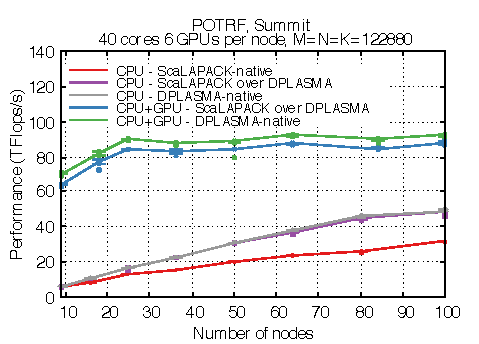
\includegraphics[width=.9\linewidth]{projects/2.3.1-PMR/2.3.1.09-ParSEC/scalapack_POTRF.pdf}
\caption{Performance using GPUs of native ScaLAPACK, ScaLAPACK over
  DPLASMA and native DPLASMA for GEMM and
  POTRF.\label{fig:scalapack_gpu}}
\end{wrapfigure}
In the context of milestone STPM11-81, the PaRSEC team worked to
enable the usage DPLASMA as a replacement for ScaLAPACK.  This
functionality is provided as an independent library which contains a
wrapped version of the ScaLAPACK API and hides the PaRSEC API from the
application while it constructs the structures necessary for the
operation with matrices represented on ScaLAPACK memory layout.  Users
of applications exploiting ScaLAPACK can link against this independent
library to run the wrapped routines over DPLASMA-PaRSEC, while any
other ScaLAPACK function, i.e. that does not have an equivalent
provided by DPLASMA, will use the original ScaLAPACK implementation.
This approach reduces to a minimum the changes that need to be
performed on the ScaLAPACK application, while enabling the
exploitation of the algorithms implemented on DPLASMA and the
operation over PaRSEC for a better exploitation of the available
hardware resources.


Figure~\ref{fig:scalapack_gpu} compare the
performance of the ScaLAPACK wrapper extensions against the native
DPLASMA and native ScaLAPACK in their typical usage scenarios (one
process per core for ScaLAPACK),
% Experiments were run using a dense matrix with dimensions 122~880 in
% double precision. The internal block size and the process grid have
% been tuned for the best performance on each library. In all cases,
% the native ScaLAPACK tests were ran spawning one process per core
while DPLASMA tests (native DPLASMA and ScaLAPACK over DPLASMA) use
one thread per core and one process per node on the experiments using
only the CPU and two processes per node, each exploiting 3 GPUs, are
used on the GPU tests.
%
In all cases, the performance achieved by running ScaLAPACK over
DPLASMA is more than 90\% the performance of native DPLASMA.  For the
CPU-only experiments, the usage of the DPLASMA wrapper introduces a
speedup of 1.73x for GEMM (minimum 1.64x, maximum 1.88x) and 1.49x for
POTRF (minimum 1.27x, maximum 1.71x) .  When exploiting also the GPUs
of the computation nodes, the performance is increased by 16.75x for
GEMM (minimum 10.79x, maximum 25.68x) and by 4.27x for POTRF (minimum
2.77x, maximum 6.70x).  The lower performance of the DPLASMA's POTRF
over GPUs is explained because in the current implementation of this
algorithm not all the tasks are run on GPUs. However, further
improvements of DPLASMA algorithms that will be integrated in the next
release of DPLASMA will likely achieved similar performance when used
for wrapping the ScaLAPACK routines. Therefore, enabling applications
already using the ScaLAPACK API to improve their usage of the
available hardware resource with very little effort that is translated
in important performance benefits.

%
% End
%


\paragraph{Recent Progress}

The software release (2021.10) provides many new additions to the low-level task
runtime, supports for a number of hardware capabilities (AMD GPUs, new device
architecture to support Intel GPUs, new communication subsystem to better
employ RDMA communications), brings significant improvements to the performance
and scalability of the runtime, and addresses many pending issues. PaRSEC
is used as the default low level task runtime for MADNESS on ECP machines.
MADNESS is the task interface and manager used by many of the applications
in the NWChemEx ECP project. The PaRSEC implementation of the TTG DSL has
been greatly improved, reaching performance comparable to other PaRSEC DSLs
and the state of the art, enabling the wide distribution of this DSL. GPU
support has been extended to the DTD DSL, enabling experiments with other
ECP applications.

%
% The installation system has been improved to take advantage of the latest
% capability of CMake, and scripts for seamless integration in the ECP software
% ecosystem (via SPack). Significant improvements have also been added on the
% performance and scalability of the runtime, as shown by the results below.
%
On the software quality side, the PaRSEC runtime has been evaluated
and amended to compile and run on all Early Access System (Arcticus
and Spock), as well as some early platforms based on the new ARM
architecture.  PaRSEC is installable through Spack on all ECP platforms,
and available as a system module on Spock.

%
% TTG
%
Template Task Graph (TTG) is a new DSL co-developed with members of
the NWChemEx team, to address issues in the other DSLs available in
PaRSEC. TTG mixes the concept original to PaRSEC of a Parameterized
Task Graph (PTG) to expose a concise and efficient representation of
the DAG of tasks, with the dynamicity and data-dependence capabilities
of the Dynamic Task Discovery paradigm that is most often used to
express task-based systems. A static graph of task classes is built
by the program at compile time, but the tasks belonging to this graph
are only instantiated at runtime. The originality of TTG lies
in the fact that task instantiation in TTG is by nature capable of
managing data dependency (i.e. depending on the computation itself a
task may or may not become instantiated), and fully distributed.
Tasks are instantiated by other tasks, while unrolling the graph of
task classes, and they do not require to expose a global knowledge on
the DAG, making the approach more scalable than usual DAG discovery.

\begin{wrapfigure}{l}{.45\linewidth}
\centering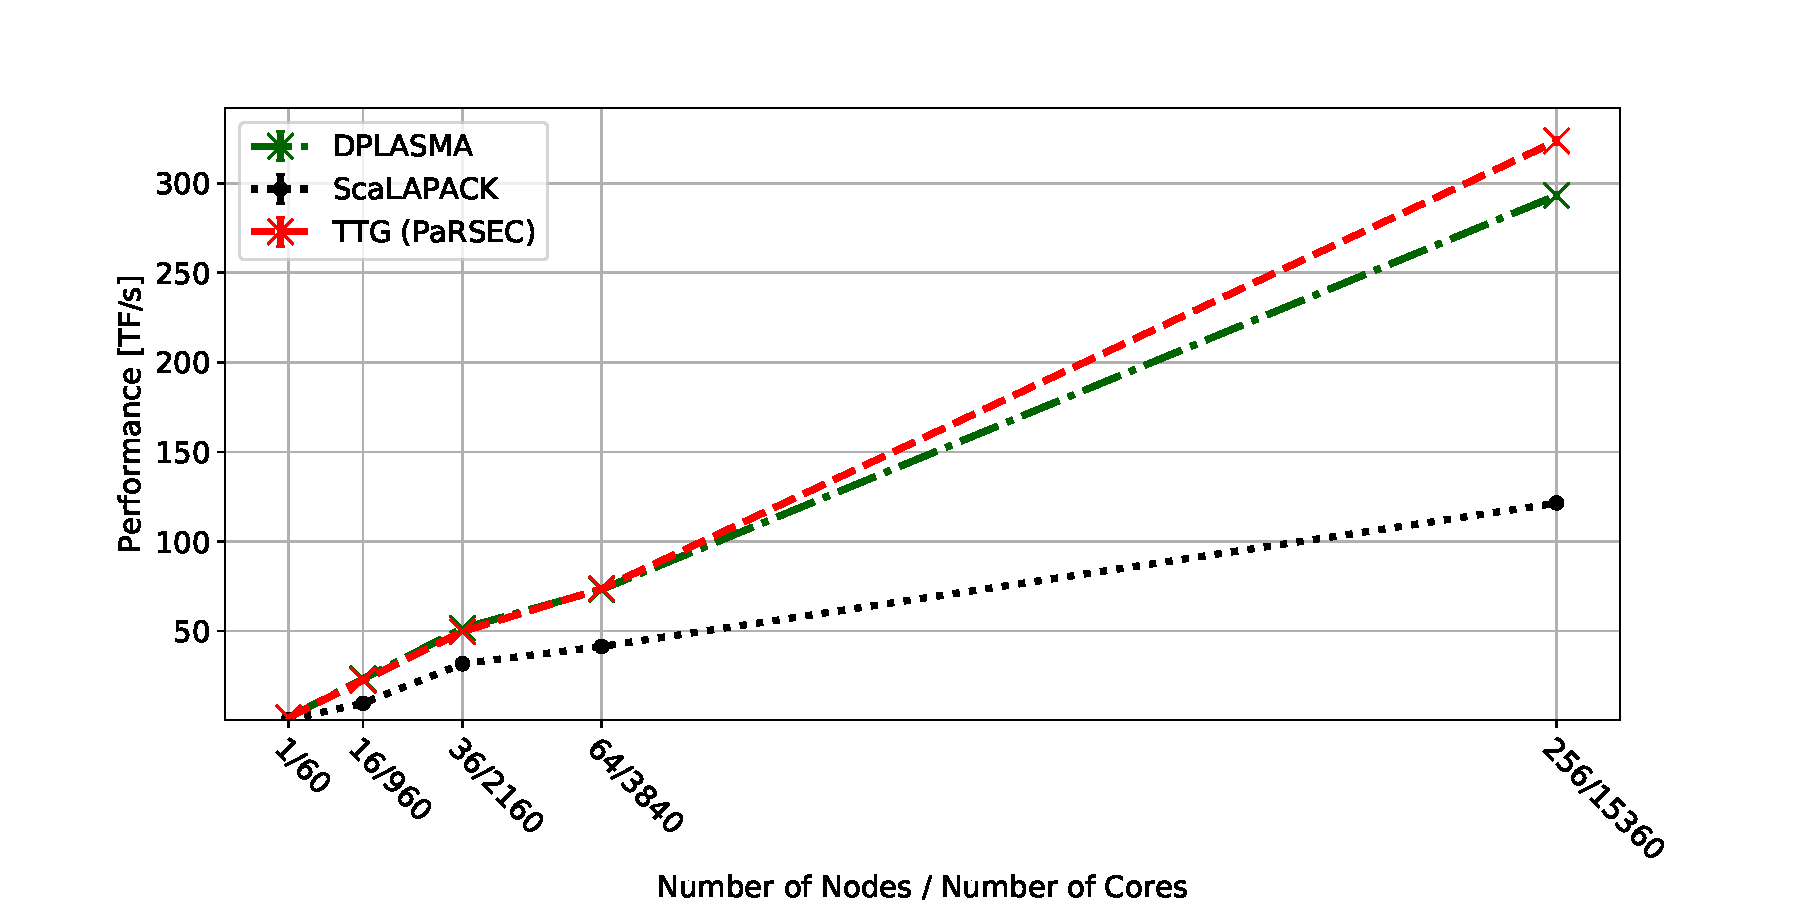
\includegraphics[width=.9\linewidth]{projects/2.3.1-PMR/2.3.1.09-ParSEC/dpotrf-ttg/dpotrf_1403612-page3.pdf}
\caption{Performance comparison between DPLASMA (PTG DSL), the TTG implementation, and ScaLAPACK, of the Cholesky factorization (double precision), for a fixed amount of memory per node (weak scaling).\label{fig:parsec:dpotrfttg:weakscale}}
\end{wrapfigure}
In the context of this collaboration, the PaRSEC team has provided
an efficient implementation of the TTG interface on top of the
PaRSEC runtime.
Figure~\ref{fig:parsec:dpotrfttg:weakscale} shows a performance
comparison on a 5,632 dual-socket 64-core AMD EPYC 7742 nodes equipped
with 256 GB main memory and connected through a Mellanox Infiniband
HDR 200 fabric, from 1 to 256 nodes (representing 15,360 cores in
total). We compare the TTG implementation of the dense Cholesky
factorization with the pdpotrf routines available in DPLASMA (thus
with the PTG implementation of the same algorithm), and in ScaLAPACK.
Each process holds a constant amount of memory, representing a
submatrix of $30k\times 30k$ elements. Each node runs 8 processes, and
each process is allocated 16 cores. With this weak-scaling experiment,
we observe that TTG behaves as efficiently and consistently as PTG. At
15,360 cores, the TTG implementation even goes slightly faster than
the PTG one, due to a better scheduling of the communications that are
discovered in a different order. Both task-based and PaRSEC-based
implementations go significantly faster than ScaLAPACK, which is the
expected behavior for a machine with so many cores per node.

%
% HIP / ROCM
%

\paragraph{Next Steps}
%\textit{Describe what you are working on next.}
% Improve DTE accelerator support and interoperability with other
% programming models
To provide programmers with more control over how accelerators are
integrated and used by the runtime, a need to provide finer control of the
resource usage by the runtime system has arisen. We are developing new APIs to
allow the programmers to advise the runtime system with respect to data
placement, prefetching, and management of cache.
%
Programming interoperability should not be limited to node-level programming
models but should extend to distributed programming. Execution modes where part
of the application is expressed in native MPI (including communicating tasks)
and other parts using PaRSEC DSLs, running above the task system in a tightly
coupled manner, are being developed.

% Facilitate DSL integration

% Provide better libraries and tools integration
The set of tools that come with the PaRSEC runtime environment to
assess performance, find bottlenecks, improve scheduling and debug the
task-based application are being improved to expose the information
in a format compatible with TAU, Score-P and other
tools that are already familiar to ECP users.
